\section{Results and Analysis}
\label{sec:results}

After the completion of the experiment programs' development, an automation mechanism was developed based on the GNU Make tool. This mechanism allowed for the repeated running of the experiments suite while also providing control over aspects such as the number of repetitions and grouping of the algorithms.

The basis for the mechanism was a series of additional rules added to the already-present ``Makefile'' files that had been developed for the building of each language's set of programs. A single target-rule, ``\texttt{experiments}'', would recursively descend into each language-specific directory and trigger all algorithms in sequence. Each algorithm ran a specified number of times, and in most cases the initial run was discarded. This was to prevent the possibility of the data input files being in the disk device's cache skewing the timing and energy readings with regards to later runs. All non-error output from the experiments was captured by the harness program and streamed to a single text file.

The format chosen for the file of results was YAML\footnote{YAML: \texttt{https://yaml.org/}}, due to the ready availability of parsing libraries. YAML had an advantage over other formats such as CSV (comma-separated values) in that it allowed the flexibility of complex nested data were it to be necessary, while also being emitted in a streaming fashion. This greatly reduced the potential for output to be corrupted between algorithm executions.

\subsection{Results from the Experiments}
\label{subsec:results}

The automated suite of experiments was run numerous times over the course of this research. The final run from which the analysis and conclusions are drawn is preserved in the same repository on the GitHub platform~\cite{github} as all the other files related to this research. The file of raw experiments data is named ``\texttt{experiments-data-20221104.yml}''.

\subsubsection{Scope of the Experiments}

The final run of the experiments generated a total of 1,190 data-points taken from runs of the 27 programs. The set of programs below includes the regular expression variants of the DFA-Gap algorithm for Perl and Python, as described in~\ref{subsubsec:dfa_regexp}. Table~\ref{table:iterations} shows the number of runs on a per-language, per-algorithm basis.

\begin{table}[h!]
\begin{center}
% Table: Algorithm iteration counts
% Generated: 2022-11-02 11:35:18.508914
\begin{tabular}{|c|c|c|c|c|c|c|}
\hline
Language&Knuth-Morris-Pratt&Boyer-Moore&Bitap&Aho-Corasick&DFA-Gap&Regexp-Gap \\
\hline
C (GCC)&25&25&25&25&10&n/a \\
C (LLVM)&25&25&25&25&10&n/a \\
C (Intel)&25&25&25&25&10&n/a \\
C++ (GCC)&25&25&25&25&10&n/a \\
C++ (LLVM)&25&25&25&25&10&n/a \\
C++ (Intel)&25&25&25&25&10&n/a \\
Rust&25&25&25&25&10&n/a \\
Perl&5&5&5&25&3&n/a \\
Python&5&5&5&25&3&n/a \\
\hline
\end{tabular}

\caption{Experiment iterations by language and algorithm}
\label{table:iterations}
\end{center}
\end{table}

For all numbers greater than or equal to 10, there was an additional ``priming'' run (as described above) to ensure that disk cache status did not play into the values for full run-time or package-level energy usage. Note also that the DFA-Gap and Regexp-Gap columns are stand-ins for 5 such columns each (for the values of $k$ from 1 to 5). Each value of $k$ was run for the same number of iterations.

\subsubsection{Outliers and the Interpreted Languages}

While it was known that the interpreted languages (Python and Perl) would be slower than the compiled languages, the reality of the results was surprising: as will be shown in section~\ref{subsec:perf_comp}, below, the interpreted languages were in some cases more than 150 times slower than the fastest compiled program on the same algorithm.

This discovery required adjusting the automated experiments, to reduce the number of iterations for both interpreted languages. The Knuth-Morris-Pratt, Boyer-Moore, and Bitap algorithms were all reduced to 5 iterations each, for these languages. The Aho-Corasick algorithm ran in a more reasonable length of time and was left at 25 iterations, the same number as were run for the compiled languages.

For the DFA-Gap algorithm, both compiled and interpreted languages had to be reduced in terms of iterations given that approximate-matching algorithms are in general slower than their exact-matching counterparts. The compiled languages ran 10 iterations of this algorithm for values of $k$ ranging from 1 to 5, whereas the interpreted languages were necessarily limited to 3 iterations for the same values of $k$.

\subsection{Performance Comparisons}
\label{subsec:perf_comp}

The first of the three measures of the languages' suitability was chosen to be the overall performance. This was chosen for first consideration as this is the metric that most developers notice first: how long did it take the program to complete?

\subsubsection{Special Casing Perl and Python}
\label{subsubsec:results:perf_perl_python}

Early examination of the performance results for Perl and Python (section~\ref{subsubsec:dfa_regexp}) had shown that the custom-built DFAs were strongly out-performed by using those languages' native support for regular expressions. Looking at these results separately from the rest of the experiments, the difference was considerable as is shown in figure~\ref{fig:graph:dfa_regexp_comp}.

\begin{figure}[h]
	\centering
	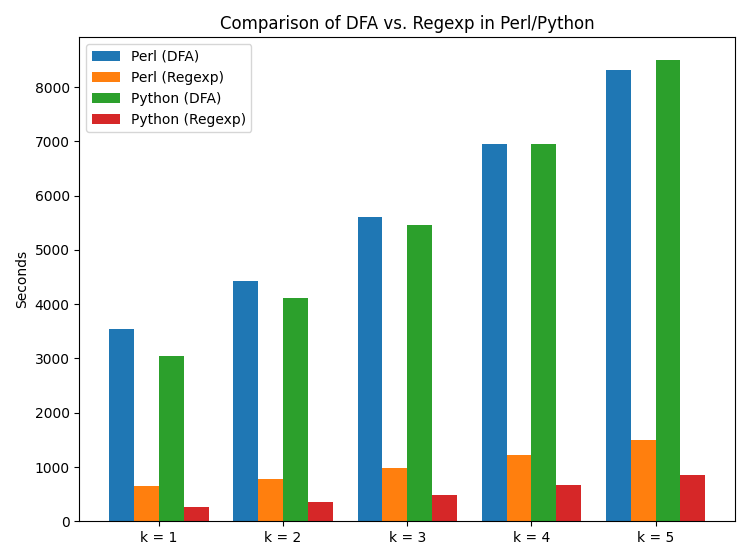
\includegraphics[width=0.85\textwidth]{figures/dfa_regexp_comp.png}
	\caption{Bar charts of DFA vs. Regexp run-times for Perl and Python}
	\label{fig:graph:dfa_regexp_comp}
\end{figure}

Not only were the run-times themselves higher for the DFA implementations, but the growth in run-time as $k$ increases was more pronounced for the DFA implementations than for the regular expression implementations. Note that while Perl's DFA was outperformed by Python's for the first three values of $k$, at $k=4$ it was effectively equal and was slightly better at $k=5$. However, in the regular expression implementation Python remained the better performer consistently.

This led to a significant question regarding the measurement of performance for the algorithms: should the Perl and Python manually-coded DFA implementations be replaced by the regular expression implementations? It is highly unlikely that an experienced programmer in either of these two languages would choose to create the DFA manually when they could instead create a regular expression based on the pattern and a given value of $k$, in any case. When the performance is so drastically disparate it seems even less likely.

\subsubsection{Collected Performance Results}

After the decision was made on the regular expression question for Perl and Python, processing of the full performance results was done. The collection of sub-tables in table~\ref{table:runtime:comparative-algorithm} shows the comparative performance of the languages on each of the algorithms. The time measurements are based on the algorithm run-time as opposed to the total run-time. In each table, the fastest language is listed first with the remaining ones following in order of performance. Run times are scaled by the fastest time. This has the result of showing each slower language's time as a percentage over the fastest.

\begin{table}[!htb]
% Table: Comparative runtimes sub-tables
% Generated: 2022-11-12 18:00:26.811341
\begin{subtable}{0.33\textwidth}
    \centering
    \caption{Knuth-Morris-Pratt}
    \label{table:runtime:kmp}
    \begin{tabular}{|l|r|}
        %% Caption: Knuth-Morris-Pratt
        %% Label: table:runtime:kmp
        %% Field(s): ['runtime']
        \hline
        Language & Score \\
        \hline
        C (LLVM) & 1.0000 \\
        Rust & 1.1293 \\
        C++ (LLVM) & 1.1377 \\
        C (Intel) & 1.1402 \\
        C++ (Intel) & 1.2406 \\
        C (GCC) & 1.3146 \\
        C++ (GCC) & 1.3350 \\
        Perl & 38.5237 \\
        Python & 41.4858 \\
        \hline
    \end{tabular}
\end{subtable}%
\begin{subtable}{0.33\textwidth}
    \centering
    \caption{Boyer-Moore}
    \label{table:runtime:boyer_moore}
    \begin{tabular}{|l|r|}
        %% Caption: Boyer-Moore
        %% Label: table:runtime:boyer_moore
        %% Field(s): ['runtime']
        \hline
        Language & Score \\
        \hline
        C (Intel) & 1.0000 \\
        C++ (Intel) & 1.0508 \\
        C (GCC) & 1.0664 \\
        Rust & 1.0977 \\
        C++ (LLVM) & 1.1413 \\
        C (LLVM) & 1.1549 \\
        C++ (GCC) & 1.1831 \\
        Perl & 46.9470 \\
        Python & 50.9587 \\
        \hline
    \end{tabular}
\end{subtable}%
\begin{subtable}{0.33\textwidth}
    \centering
    \caption{Bitap}
    \label{table:runtime:shift_or}
    \begin{tabular}{|l|r|}
        %% Caption: Bitap
        %% Label: table:runtime:shift_or
        %% Field(s): ['runtime']
        \hline
        Language & Score \\
        \hline
        C (Intel) & 1.0000 \\
        C (GCC) & 1.0068 \\
        C++ (Intel) & 1.0475 \\
        C (LLVM) & 1.1219 \\
        Rust & 1.1350 \\
        C++ (GCC) & 1.1616 \\
        C++ (LLVM) & 1.2381 \\
        Perl & 155.3435 \\
        Python & 192.9283 \\
        \hline
    \end{tabular}
\end{subtable}
\begin{subtable}{0.33\textwidth}
    \centering
    \caption{Aho-Corasick}
    \label{table:runtime:aho_corasick}
    \begin{tabular}{|l|r|}
        %% Caption: Aho-Corasick
        %% Label: table:runtime:aho_corasick
        %% Field(s): ['runtime']
        \hline
        Language & Score \\
        \hline
        C (LLVM) & 1.0000 \\
        C (Intel) & 1.0443 \\
        C (GCC) & 1.0644 \\
        C++ (GCC) & 1.1519 \\
        C++ (LLVM) & 1.1600 \\
        Rust & 1.1816 \\
        C++ (Intel) & 1.1988 \\
        Python & 19.7040 \\
        Perl & 39.4041 \\
        \hline
    \end{tabular}
\end{subtable}%
\begin{subtable}{0.33\textwidth}
    \centering
    \caption{DFA-Gap (k=3)}
    \label{table:runtime:dfa_gap}
    \begin{tabular}{|l|r|}
        %% Caption: DFA-Gap (k=3)
        %% Label: table:runtime:dfa_gap
        %% Field(s): ['runtime']
        \hline
        Language & Score \\
        \hline
        C (GCC) & 1.0000 \\
        C (LLVM) & 1.0749 \\
        C (Intel) & 1.1561 \\
        C++ (GCC) & 1.2270 \\
        C++ (LLVM) & 1.3250 \\
        C++ (Intel) & 1.3443 \\
        Rust & 1.7632 \\
        Perl & 56.2209 \\
        Python & 57.4437 \\
        \hline
    \end{tabular}
\end{subtable}%
\begin{subtable}{0.33\textwidth}
    \centering
    \caption{Regexp-Gap (k=3)}
    \label{table:runtime:regexp}
    \begin{tabular}{|l|r|}
        %% Caption: Regexp-Gap (k=3)
        %% Label: table:runtime:regexp
        %% Field(s): ['runtime']
        \hline
        Language & Score \\
        \hline
        Rust & 1.0000 \\
        C++ (LLVM) & 1.1747 \\
        C++ (GCC) & 1.1753 \\
        C++ (Intel) & 1.1794 \\
        C (Intel) & 1.2871 \\
        C (GCC) & 1.2876 \\
        C (LLVM) & 1.2888 \\
        Python & 1.7398 \\
        Perl & 3.9966 \\
        \hline
    \end{tabular}
\end{subtable}

\caption{Comparative run-times by algorithm}
\label{table:runtime:comparative-algorithm}
\end{table}

The DFA-Gap algorithm is shown for all values of $k$ that were used, as it is interesting to see the subtle differences in the ranking of languages for different values of $k$.

\subsection{Energy Usage Comparisons}
\label{subsec:energy_comp}

In this section the energy usage results are examined. Table~\ref{table:energy:comparative-algorithm} shows the comparative energy usage over time (Joules per second) for each algorithm with the same scaling methodology applied as was used for the performance tables. The tables here use the ``Package'' and ``DRAM'' energy values combined together, divided by total run-time.

\begin{table}[!htb]
% Table: Comparative energy usage sub-tables
% Generated: 2022-11-11 19:03:08.364288
\begin{subtable}{0.33\textwidth}
    \centering
    \caption{Knuth-Morris-Pratt}
    \label{table:energy:kmp}
    \begin{tabular}{|l|r|}
        %% Caption: Knuth-Morris-Pratt
        %% Label: table:energy:kmp
        %% Field(s): ['package', 'dram']
        %% Divisor(s): ['total_runtime']
        \hline
        Language & Score \\
        \hline
        Rust & 1.0000 \\
        C (GCC) & 1.0403 \\
        C (LLVM) & 1.0756 \\
        C (Intel) & 1.0786 \\
        C++ (GCC) & 1.0983 \\
        C++ (LLVM) & 1.1033 \\
        C++ (Intel) & 1.1102 \\
        Python & 1.1651 \\
        Perl & 1.2957 \\
        \hline
    \end{tabular}
\end{subtable}%
\begin{subtable}{0.33\textwidth}
    \centering
    \caption{Boyer-Moore}
    \label{table:energy:boyer_moore}
    \begin{tabular}{|l|r|}
        %% Caption: Boyer-Moore
        %% Label: table:energy:boyer_moore
        %% Field(s): ['package', 'dram']
        %% Divisor(s): ['total_runtime']
        \hline
        Language & Score \\
        \hline
        C++ (GCC) & 1.0000 \\
        C++ (LLVM) & 1.0115 \\
        Rust & 1.0331 \\
        C (GCC) & 1.0358 \\
        C++ (Intel) & 1.0747 \\
        C (LLVM) & 1.0918 \\
        C (Intel) & 1.1501 \\
        Python & 1.2985 \\
        Perl & 1.3103 \\
        \hline
    \end{tabular}
\end{subtable}%
\begin{subtable}{0.33\textwidth}
    \centering
    \caption{Bitap}
    \label{table:energy:shift_or}
    \begin{tabular}{|l|r|}
        %% Caption: Bitap
        %% Label: table:energy:shift_or
        %% Field(s): ['package', 'dram']
        %% Divisor(s): ['total_runtime']
        \hline
        Language & Score \\
        \hline
        C++ (LLVM) & 1.0000 \\
        C (Intel) & 1.0049 \\
        Rust & 1.0077 \\
        C (LLVM) & 1.0101 \\
        C++ (Intel) & 1.0440 \\
        Python & 1.0799 \\
        C++ (GCC) & 1.0854 \\
        C (GCC) & 1.0897 \\
        Perl & 1.2268 \\
        \hline
    \end{tabular}
\end{subtable}
\begin{subtable}{0.33\textwidth}
    \centering
    \caption{Aho-Corasick}
    \label{table:energy:aho_corasick}
    \begin{tabular}{|l|r|}
        %% Caption: Aho-Corasick
        %% Label: table:energy:aho_corasick
        %% Field(s): ['package', 'dram']
        %% Divisor(s): ['total_runtime']
        \hline
        Language & Score \\
        \hline
        C++ (LLVM) & 1.0000 \\
        C (Intel) & 1.0303 \\
        C (GCC) & 1.0332 \\
        C (LLVM) & 1.0448 \\
        C++ (Intel) & 1.0471 \\
        C++ (GCC) & 1.0813 \\
        Rust & 1.0939 \\
        Perl & 1.1248 \\
        Python & 1.1736 \\
        \hline
    \end{tabular}
\end{subtable}%
\begin{subtable}{0.33\textwidth}
    \centering
    \caption{DFA-Gap (k=3)}
    \label{table:energy:dfa_gap(3)}
    \begin{tabular}{|l|r|}
        %% Caption: DFA-Gap (k=3)
        %% Label: table:energy:dfa_gap(3)
        %% Field(s): ['package', 'dram']
        %% Divisor(s): ['total_runtime']
        \hline
        Language & Score \\
        \hline
        Rust & 1.0000 \\
        C++ (LLVM) & 1.1603 \\
        C (LLVM) & 1.1812 \\
        C++ (Intel) & 1.2078 \\
        C (Intel) & 1.2231 \\
        C (GCC) & 1.2352 \\
        C++ (GCC) & 1.2497 \\
        Python & 1.3140 \\
        Perl & 1.3897 \\
        \hline
    \end{tabular}
\end{subtable}%
\begin{subtable}{0.33\textwidth}
    \centering
    \caption{Regexp-Gap (k=3)}
    \label{table:energy:regexp(3)}
    \begin{tabular}{|l|r|}
        %% Caption: Regexp-Gap (k=3)
        %% Label: table:energy:regexp(3)
        %% Field(s): ['package', 'dram']
        %% Divisor(s): ['total_runtime']
        \hline
        Language & Score \\
        \hline
        C (Intel) & 1.0000 \\
        C (GCC) & 1.0055 \\
        C (LLVM) & 1.0094 \\
        C++ (LLVM) & 1.0428 \\
        C++ (GCC) & 1.0460 \\
        C++ (Intel) & 1.0473 \\
        Perl & 1.0513 \\
        Rust & 1.0561 \\
        Python & 1.0618 \\
        \hline
    \end{tabular}
\end{subtable}

\caption{Comparative energy usage over time by algorithm}
\label{table:energy:comparative-algorithm}
\end{table}

The language exhibiting the lowest energy usage is listed first, with the rest ranked behind it. The DFA-Gap algorithm is again represented for all values of $k$, as the ranking of languages varies with $k$.

These results are further illustrated by figure~\ref{fig:graph:power_per_sec}. In this collection of bar-charts, the Rust language (represented by the pink bars) can be seen to be the lowest value in the Knuth-Morris-Pratt, Boyer-Moore, and DFA-Gap instances. In fact, Rust scored the lowest energy usage for all five variations of the DFA-Gap algorithm, making it the most-efficient language for 7 of the 9 distinct groups of experiments.

\begin{figure}
	\centering
	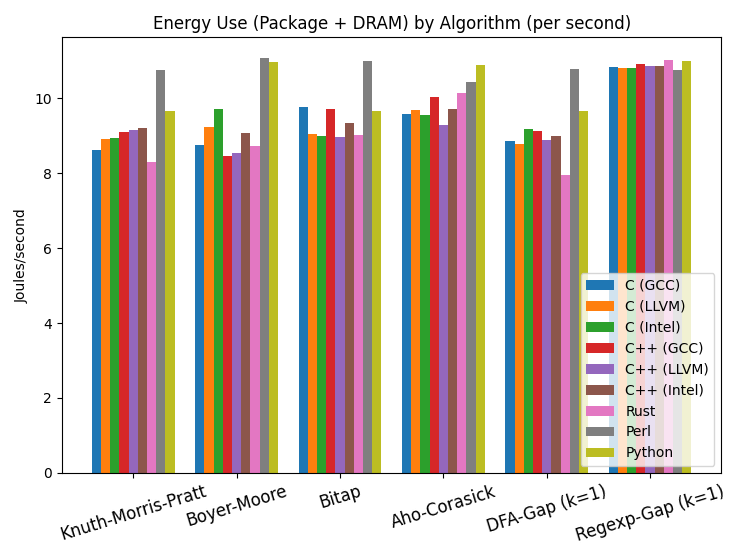
\includegraphics[width=0.85\textwidth]{figures/power_per_sec.png}
	\caption{Bar charts of energy usage per second, by algorithm}
	\label{fig:graph:power_per_sec}
\end{figure}

\subsection{Expressiveness Comparisons}
\label{subsec:expr_comp}

In comparing expressiveness, it is useful to look at all three of the chosen comparative measures in an aggregated fashion. First, the individual numbers will be examined. As with the previous two bases, tables will show the numbers comparing the languages. Unlike the previous sections, the numbers shown will be for the combined files of all algorithm modules, as well as runner modules and input modules. For each language the source code was combined in a way that facilitated each of the metrics:

\begin{description}
\item[SLOC:] Total SLOC values for each language's files were combined. In the case of C and C++, this includes relevant lines from the header files for the runner and input modules.
\item[Complexity:] Each file's cyclomatic complexity values were computed on a per-function basis. Any function whose value was exactly 1 was discarded so as to not artificially lower the average complexity for the module. Each module's function-level scores were then averaged, and all modules' averages for a given language were summed together.
\item[Conciseness:] Using a method adapted from Bergmans, et al~\cite{bergmans}, each source code file for a given language was stripped of comments and then merged into a sort of ``archive'' using the standard ``\texttt{cat}'' command available on Linux. Each such resulting file was then compressed with the ``\texttt{xz}'' compression utility and the compression ratio recorded.
\end{description}

\subsubsection{Source Lines of Code}

In table~\ref{table:expr:sloc}, the SLOC totals are shown in three sub-tables: only the algorithm implementations, then the framework totals, and finally the combined totals of all lines.

\begin{table}[!htb]
% Table: Comparative SLOC totals sub-tables
% Generated: 2022-11-04 19:01:11.807483
\begin{subtable}{0.33\textwidth}
    \centering
    \begin{tabular}{|c|r|r|}
        \hline
        Language & Code & Score \\
        \hline
        Python & 257 & 1.0000 \\
        Perl & 354 & 1.3774 \\
        C++ & 368 & 1.4319 \\
        C & 473 & 1.8405 \\
        Rust & 507 & 1.9728 \\
        \hline
    \end{tabular}
    \caption{Algorithm lines}
    \label{table:sloc:algorithm}
\end{subtable}%
\begin{subtable}{0.33\textwidth}
    \centering
    \begin{tabular}{|c|r|r|}
        \hline
        Language & Support & Score \\
        \hline
        Python & 148 & 1.0000 \\
        Perl & 211 & 1.4257 \\
        C++ & 266 & 1.7973 \\
        Rust & 272 & 1.8378 \\
        C & 353 & 2.3851 \\
        \hline
    \end{tabular}
    \caption{Framework lines}
    \label{table:sloc:framework}
\end{subtable}%
\begin{subtable}{0.33\textwidth}
    \centering
    \begin{tabular}{|c|r|r|}
        \hline
        Language & All & Score \\
        \hline
        Python & 405 & 1.0000 \\
        Perl & 565 & 1.3951 \\
        C++ & 634 & 1.5654 \\
        Rust & 779 & 1.9235 \\
        C & 826 & 2.0395 \\
        \hline
    \end{tabular}
    \caption{Total of lines}
    \label{table:sloc:all}
\end{subtable}

\caption{Comparison of SLOC by language}
\label{table:expr:sloc}
\end{table}

Here Python is the clear leader, with Perl being 40\% larger in table~\ref{table:sloc:all}. C++ maintains the third-place ranking across all three sub-tables, and Rust edges out C in both the framework measurement and the total lines measurement. Rust's score in table~\ref{table:sloc:algorithm} likely suffered from the necessary mechanism that was used to pass and unpack pattern representation between a given algorithm's initialization function and the algorithm function itself. Compare the listings, below.

\begin{lstlisting}[language=C,caption={C unpacking of pattern data},label={lst:c_unpack}]
    int *pattern_count = (int *)pat_data[0];
    int *goto_fn = (int *)pat_data[1];
    int *failure_fn = (int *)pat_data[2];
    Set *output_fn = (Set *)pat_data[3];
\end{lstlisting}


\begin{lstlisting}[language=Rust,caption={Rust unpacking of pattern data},label={lst:rust_unpack},showstringspaces=false]
    let pattern_count = match &pat_data[0] {
        MultiPatternData::PatternCount(val) => val,
        _ => panic!("Incorrect value at pat_data slot 0"),
    };
    let goto_fn = match &pat_data[1] {
        MultiPatternData::PatternIntVecVec(val) => val,
        _ => panic!("Incorrect value at pat_data slot 1"),
    };
    let failure_fn = match &pat_data[2] {
        MultiPatternData::PatternUsizeVec(val) => val,
        _ => panic!("Incorrect value at pat_data slot 2"),
    };
    let output_fn = match &pat_data[3] {
        MultiPatternData::PatternTypeVec(val) => val,
        _ => panic!("Incorrect value at pat_data slot 3"),
    };
\end{lstlisting}


In this area, C and C++ each needed only one line per element passed (listing~\ref{lst:c_unpack}), while Rust required four\footnote{One of which was a closing-brace with a semicolon and might not have been counted by the \texttt{sloc} tool} (listing~\ref{lst:rust_unpack}). This is a 12-line difference in just the Aho-Corasick implementation, so it can be understood how this would likely propagate through the other five algorithm implementations.

By further comparison: both Python and Perl, having the native ability to pass arrays of differing types, needed only one line to unpack the pattern representations.

\subsubsection{Cyclomatic Complexity}

Table~\ref{table:expr:cyclomatic} shows a similar break-down of the cyclomatic complexity measurements: algorithms, framework, and combined total.

\begin{table}[!htb]
% Table: Comparative cyclomatic totals sub-tables
% Generated: 2022-11-12 18:00:26.813913
\begin{subtable}{0.33\textwidth}
    \centering
    \caption{Algorithms complexity}
    \label{table:cyclomatic:algorithm}
    \begin{tabular}{|c|r|r|}
        \hline
        Language & Total & Avg \\
        \hline
        Python & 76 & 19.57 \\
        C++ & 81 & 16.83 \\
        Perl & 106 & 26.97 \\
        C & 114 & 18.30 \\
        Rust & 132 & 17.97 \\
        \hline
    \end{tabular}
\end{subtable}%
\begin{subtable}{0.33\textwidth}
    \centering
    \caption{Framework complexity}
    \label{table:cyclomatic:framework}
    \begin{tabular}{|c|r|r|}
        \hline
        Language & Total & Avg \\
        \hline
        C++ & 43 & 10.75 \\
        Python & 47 & 9.90 \\
        Rust & 58 & 5.43 \\
        Perl & 61 & 12.90 \\
        C & 76 & 19.00 \\
        \hline
    \end{tabular}
\end{subtable}%
\begin{subtable}{0.33\textwidth}
    \centering
    \caption{Total complexity}
    \label{table:cyclomatic:total}
    \begin{tabular}{|c|r|r|}
        \hline
        Language & Total & Avg \\
        \hline
        Python & 123 & 29.47 \\
        C++ & 124 & 27.58 \\
        Perl & 167 & 39.87 \\
        C & 190 & 37.30 \\
        Rust & 190 & 23.40 \\
        \hline
    \end{tabular}
\end{subtable}

\caption{Comparison of complexity by language}
\label{table:expr:cyclomatic}
\end{table}

Unlike the SLOC measurements, however, there is greater variation in the rankings of the languages. Here the contest between the first and second rankings was between Python and C++. Rust placed last in the measure of the algorithm code, possibly due to the same issue of excess lines around the unpacking of pattern data. Rust did rank third in the framework table~\ref{table:cyclomatic:framework} where it also had a significantly lower average value than C++ or Python. Even as Rust ended tied for the fourth rank in the total table, its totaled average complexity was still the lowest of the five.

It is important here to note again that it was necessary to use different tools to calculate the complexity of the Perl and Rust code. The \texttt{lizard} tool did not support Perl at all, and examination of the Rust results showed some bugs in the handling of Rust. Because of this, it is not possible to say with certainty that the relative comparisons of complexity between the five languages are completely sound. For the purposes of this paper the total complexity values will be used as presented here. It is felt that this will be sufficient as these values will only contribute $\frac{1}{3}$ of the value of the final expressiveness value.

\subsubsection{Conciseness}
\label{subsubsec:conciseness}

Conciseness proved to be a difficult concept to quantify. The approach taken in~\cite{bergmans} was designed around a significantly larger database of source code, but as the results from that paper were compelling it led to the adaptation of a variation of that methodology here.

The steps for deriving this measurement were:

\begin{enumerate}
\item A clean copy of all source code was made into a series of directories named by language
\item All comments and blank lines were removed by the \texttt{cloc} tool
\item Each individual language directory had all text files concatenated into a single file
\item Each of these text files were compressed with \texttt{xv} and the compression ratio recorded
\end{enumerate}

A key difference between~\ref{bergmans} and here is the limited scope of the data being analyzed; since there is essentially just one ``project'' being put to scrutiny, the results are sensitive to the fact that some of the files were smaller in size to begin with. Initially the technique in~\cite{bergmans} was followed exactly, and involved using the standard \texttt{tar} utility to create the archives of each language. But when put into practice it was found that the metadata overhead of a \texttt{tar} archive was more than the size of the actual data in some cases.

Further, in their paper, Bergmans and their team had removed most smaller examples of code for each language from the final measurements. This was not an option here given the limited size and number of the samples. For this reason the decision was made to focus the compression on the text content only, by applying concatenation to the stripped versions of the source files and compressing the results of this process.

In table~\ref{table:expr:compression}, the results are shown.

\begin{table}[!htb]
% Table: Compression ratios table
% Generated: 2022-11-11 19:03:08.366214
\centering
\begin{tabular}{|l|c|c|}
    \hline
    Language & Ratio & Score \\
    \hline
    Python & 78.50\% & 1.0000 \\
    Perl & 80.50\% & 1.0255 \\
    C & 80.60\% & 1.0268 \\
    Rust & 80.80\% & 1.0293 \\
    C++ & 81.00\% & 1.0318 \\
    \hline
\end{tabular}

\caption{Comparison of compressibility}
\label{table:expr:compression}
\end{table}

The ranking of Python and Perl as the first two is expected. However, the placing of C ahead of both Rust and C++ came as a surprise given the presence of highly-repetitive calls to library routines for the manual memory management. However, C and Rust both likely benefited from the need for additional support code in the Aho-Corasick algorithm which could have brought the compression ratio slightly further down. Lastly, as with the previous two metrics, it is likely that Rust was effectively penalized for the very verbose and detailed blocks that were necessary for passing the processed pattern data between initialization and algorithm functions.

\subsubsection{Combining the Expressiveness Metrics}

At this point the next step was to derive a single measurement of expressiveness from the three measurements taken. For this, it would be needed to have ``score'' values for cyclomatic complexity that were in line with the scores computed for SLOC and conciseness. These values were computed from table~\ref{table:cyclomatic:total} and are shown in table~\ref{table:expr:cyclomatic-score}.

\begin{table}[!htb]
% Table: Cyclomatic scores for all files
% Generated: 2022-11-11 19:03:08.367054
\centering
\begin{tabular}{|l|r|r|}
    \hline
    Language & Total & Score \\
    \hline
    Python & 123 & 1.0000 \\
    C++ & 124 & 1.0081 \\
    Perl & 167 & 1.3577 \\
    C & 190 & 1.5447 \\
    Rust & 190 & 1.5447 \\
    \hline
\end{tabular}

\caption{Scoring of the cyclomatic complexity results}
\label{table:expr:cyclomatic-score}
\end{table}

Here, the score shows a virtual tie for first position between C++ and Python. Their gap is just one point (less than 1\%), while the next gap is 43 (an increase of almost 35\%).

Now it would be possible to utilize the three expressiveness metrics to calculate a single value for each language. The following values would be combined into a series of 3-element vectors for each language:

\begin{itemize}
\item The SLOC scores from table~\ref{table:sloc:all}, the total of lines
\item The cyclomatic scores from table~\ref{table:expr:cyclomatic-score}
\item The conciseness scores from table~\ref{table:expr:compression}
\end{itemize}

These vectors' lengths were calculated and scaled by the lowest value, giving the values in table~\ref{table:expr:expressiveness-score}:

\begin{table}[!htb]
% Table: Calculated expressiveness score
% Generated: 2022-11-07 19:21:37.618600
\centering
\begin{tabular}{|l|r|r|r|r|}
    \hline
    \thead{Language} & \thead{SLOC} & \thead{Complexity} & \thead{Compression} & \thead{Score} \\
    \hline
    Python & 1.0000 & 1.0000 & 1.0000 & 1.0000 \\
    C++ & 1.6000 & 1.0081 & 1.0318 & 1.1565 \\
    Perl & 1.3976 & 1.3577 & 1.0255 & 1.2109 \\
    Rust & 1.9405 & 1.5447 & 1.0293 & 1.4086 \\
    C & 2.0976 & 1.5447 & 1.0268 & 1.4503 \\
    \hline
\end{tabular}

\caption{Calculated expressiveness score}
\label{table:expr:expressiveness-score}
\end{table}

It was not a surprise that Python ended up ranked as the most-expressive of the five contenders, as it had led the group in all three expressiveness metrics. The ranking of C++ ahead of Perl by just over 5 percentage points was more of a surprise, while the presence of C at the bottom was also not surprising.

Because of the possibly-inconsistent nature of the complexity data, it was decided to derive a second score based on just the SLOC and compression scores. All other calculation steps were the same. This resulted in table~\ref{table:expr:expressiveness-score2}.

\begin{table}[!htb]
% Table: Calculated expressiveness score (2-axis)
% Generated: 2022-11-11 19:03:10.009923
\centering
\begin{tabular}{|l|r|r|r|}
    \hline
    \thead{Language} & \thead{SLOC} & \thead{Compression} & \thead{Score} \\
    \hline
    Python & 1.0000 & 1.0000 & 1.0000 \\
    Perl & 1.3976 & 1.0255 & 1.1406 \\
    C++ & 1.6000 & 1.0318 & 1.2159 \\
    Rust & 1.9405 & 1.0293 & 1.3446 \\
    C & 2.0976 & 1.0268 & 1.4070 \\
    \hline
\end{tabular}

\caption{Calculated expressiveness score, 2-axis}
\label{table:expr:expressiveness-score2}
\end{table}

Here, the results more closely track with expectations: Python and Perl head the list while C++ and Rust take the next two places. As has been mentioned, it is possible that Rust most likely suffered in the SLOC measurement due to the data-unpacking mechanism required by the framework.

\subsection{Combining the Bases}
\label{subsec:combined}
